\documentclass{article}
\usepackage[utf8]{inputenc}
\usepackage{authblk}
\usepackage{setspace}
\usepackage[margin=1.25in]{geometry}
\usepackage{graphicx}
\usepackage{xcolor}
\usepackage{float}
\graphicspath{ {./figures/} }
\usepackage{amsmath,amssymb,amsfonts}
\usepackage{booktabs}
\usepackage{natbib}
\usepackage{hyperref}
\hypersetup{colorlinks=true, linkcolor=blue, citecolor=blue, urlcolor=blue}

\title{\textbf{Valuation and Subsequent Returns in Vietnam: Does a Low Market P/E Predict Higher One-Year VN-Index Returns?}}
\author[1]{SIQuant Research}
\affil[1]{Hypothesis $\times$ Quant}
\date{\today}
\onehalfspacing

\begin{document}
\maketitle

\begin{abstract}
\noindent \textbf{Hypothesis:} $H_0$: the VN-Index P/E has no predictive power for the 252-session-ahead VN-Index return; $H_1$: the slope is negative \\
\textbf{Data:} 2,033 daily observations, 2017-08-24 to 2025-10-15; P/E range 9.6 to 20.1 \\
\textbf{Method:} OLS with Newey--West HAC errors (252 lags) and a 2,000-draw circular-shift placebo; the decision needs both one-sided $p<0.05$ \\
\textbf{Results:} $\beta=-0.0541$ (HAC $t=-3.23$, $p=0.0006$; placebo $p=0.0005$), $R^2=0.231$. \\
\textbf{Research decision:} \colorbox[rgb]{0.10,0.50,0.20}{\textcolor{white}{\textbf{\,ACCEPTED\,}}}
\end{abstract}

\section{Design}
Valuation ratios are a classical predictor of long-horizon returns \citep{campbell1988stock}. The P/E at the close of day $t$ is paired with the log return over the following 252 sessions; the overlap makes the HAC lag equal to the horizon and the circular-shift placebo is the main robustness check.

\section{Results}
\begin{figure}[H]
\centering
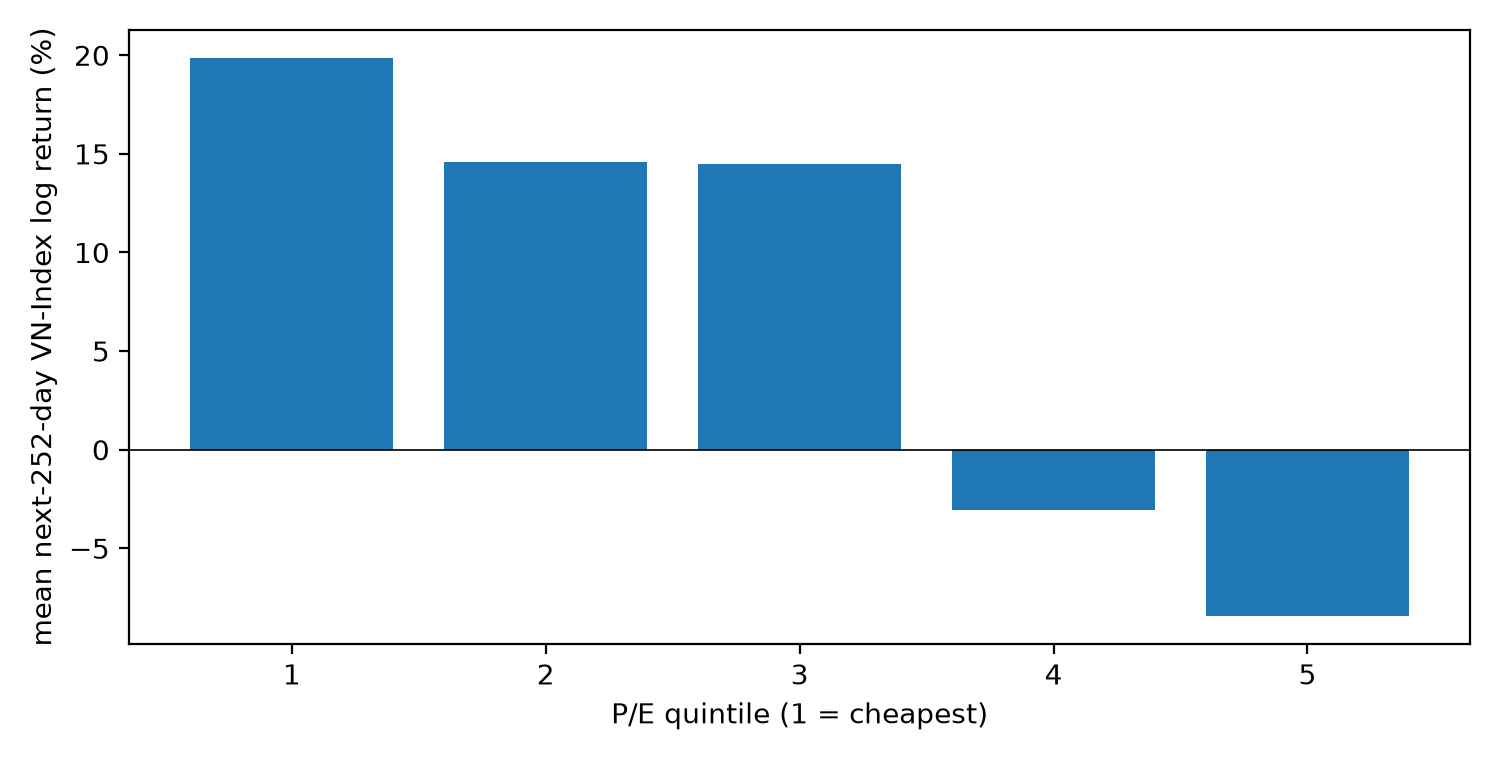
\includegraphics[width=0.8\textwidth]{fig1_pe_quintile_forward_return.png}
\caption{Mean one-year-ahead VN-Index return by P/E quintile.}
\end{figure}

\section{Limitations}
The sample holds about eight non-overlapping years, so the effective sample is under ten independent observations; the P/E uses trailing earnings which are reported with a lag and may be revised, a point-in-time earnings series is not free.


\bibliographystyle{plainnat}
\bibliography{references}

\end{document}
